\documentclass{standalone}

\usepackage{tkz-euclide}
\usepackage{animate} % Balíček pro animace
\usepackage{ifthen}  % Balíček pro podmínky

\begin{document}

% Nastavení animace:
% controls = zobrazí tlačítka play/stop
% loop = smyčka jede stále dokola
% 1 = počet snímků za sekundu (zde 1 snímek za vteřinu, aby se to dalo stíhat sledovat)
\begin{animateinline}[controls, autoplay, loop]{2}
    
    % Začátek smyčky pro 7 snímků (i = 1 až 7)
    \multiframe{7}{i=1+1}{
        
        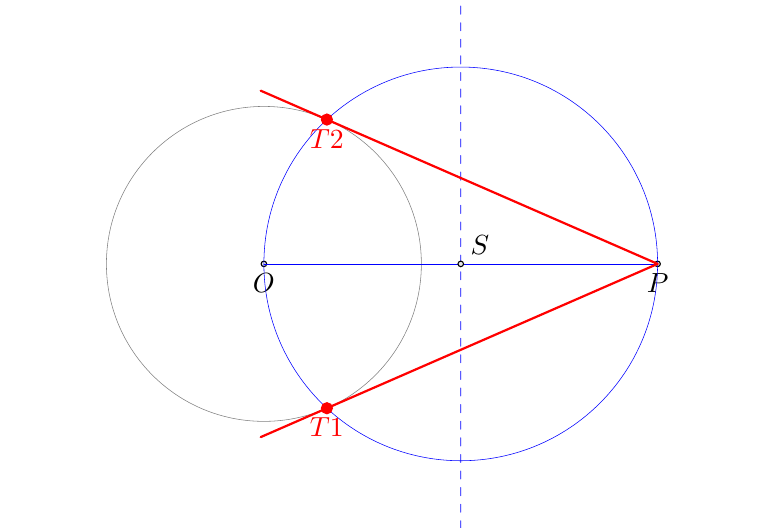
\begin{tikzpicture}[scale=1]
            % 1. FIXNÍ RÁMEČEK (Velmi důležité!)
            % Bez tohoto by obrázek "skákal", jak by se zvětšoval.
            % Definuje pevný prostor, ve kterém se animace odehrává.
            \useasboundingbox (-3,-3) rectangle (6,3);

            % --- DEFINICE BODŮ (Počítají se vždy na pozadí) ---
            \tkzDefPoint(0,0){O}
            \tkzDefPoint(0,2){r} % Pomocný bod pro poloměr
            \tkzDefPoints{5/0/P}
            \tkzDefLine[mediator](O,P) \tkzGetPoints{md1}{md2}
            \tkzInterLL(O,P)(md1,md2) \tkzGetPoint{S}
            \tkzInterCC(S,P)(O,r) \tkzGetPoints{T1}{T2}

            % --- STÁLÉ PRVKY (Vykreslí se v každém snímku) ---
            \tkzDrawCircle(O,r)
            \tkzDrawPoints(O,P)
            \tkzLabelPoints(O,P)
            
            % --- PODMÍNĚNÉ VYKRESLOVÁNÍ ---
            % Proměnná \i nese číslo aktuálního snímku.
            
            % KROK 2 a více: Spojnice OP
            \ifnum \i > 1
                \tkzDrawSegment[color=blue](O,P)
            \fi

            % KROK 3 až 5: Konstrukční oblouky (pak zmizí, aby nerušily)
            \ifnum \i > 2
                \ifnum \i < 6
                    \tkzCompass[color=gray, length=1.5](P,md1)
                    \tkzCompass[color=gray, length=1.5](P,md2)
                    \tkzCompass[color=gray, length=1.5](O,md1)
                    \tkzCompass[color=gray, length=1.5](O,md2)
                \fi
            \fi

            % KROK 4 a více: Osa úsečky a střed S
            \ifnum \i > 3
                \tkzDrawSegment[dashed,color=blue](md1,md2)
                \tkzDrawPoint(S)
                \tkzLabelPoint[above right](S){$S$}
            \fi

            % KROK 5 a více: Thaletova kružnice
            \ifnum \i > 4
                \tkzDrawCircle[color=blue](S,P)
            \fi

            % KROK 6 a více: Body dotyku
            \ifnum \i > 5
                \tkzDrawPoints[color=red, size=4](T1,T2)
                \tkzLabelPoints[color=red](T1,T2)
            \fi

            % KROK 7: Výsledné tečny
            \ifnum \i > 6
                \tkzDrawLines[thick, color=red, add=0 and 0.2](P,T1 P,T2)
            \fi

        \end{tikzpicture}
    }
\end{animateinline}

\end{document}